\chapter{Results}

\section{Unsupervised Testing}

\begin{figure}%
    \centering
    \subfloat[\centering Isolation Forest]{{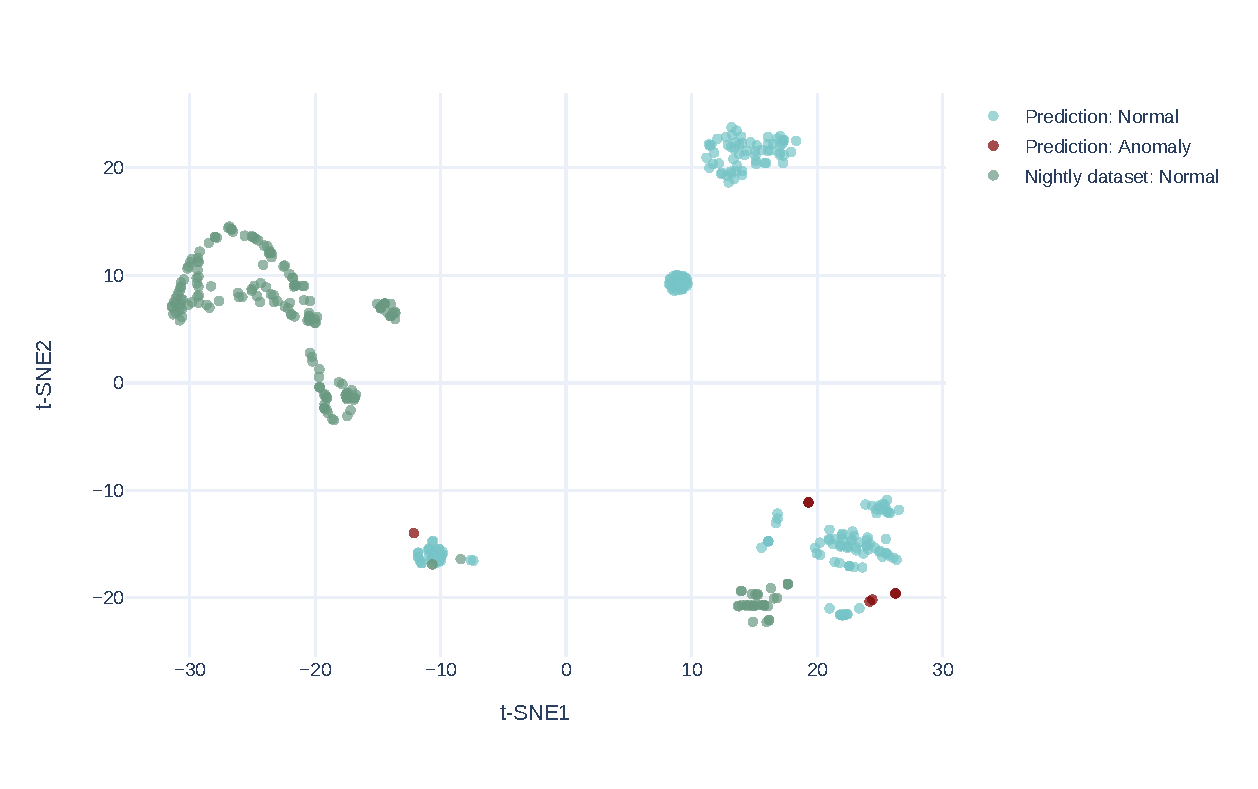
\includegraphics[width=0.9\textwidth]{img/tsne-predictions-unlabeled-isolation-forest.pdf} }}%
    \qquad
    \subfloat[\centering Invariants Mining]{{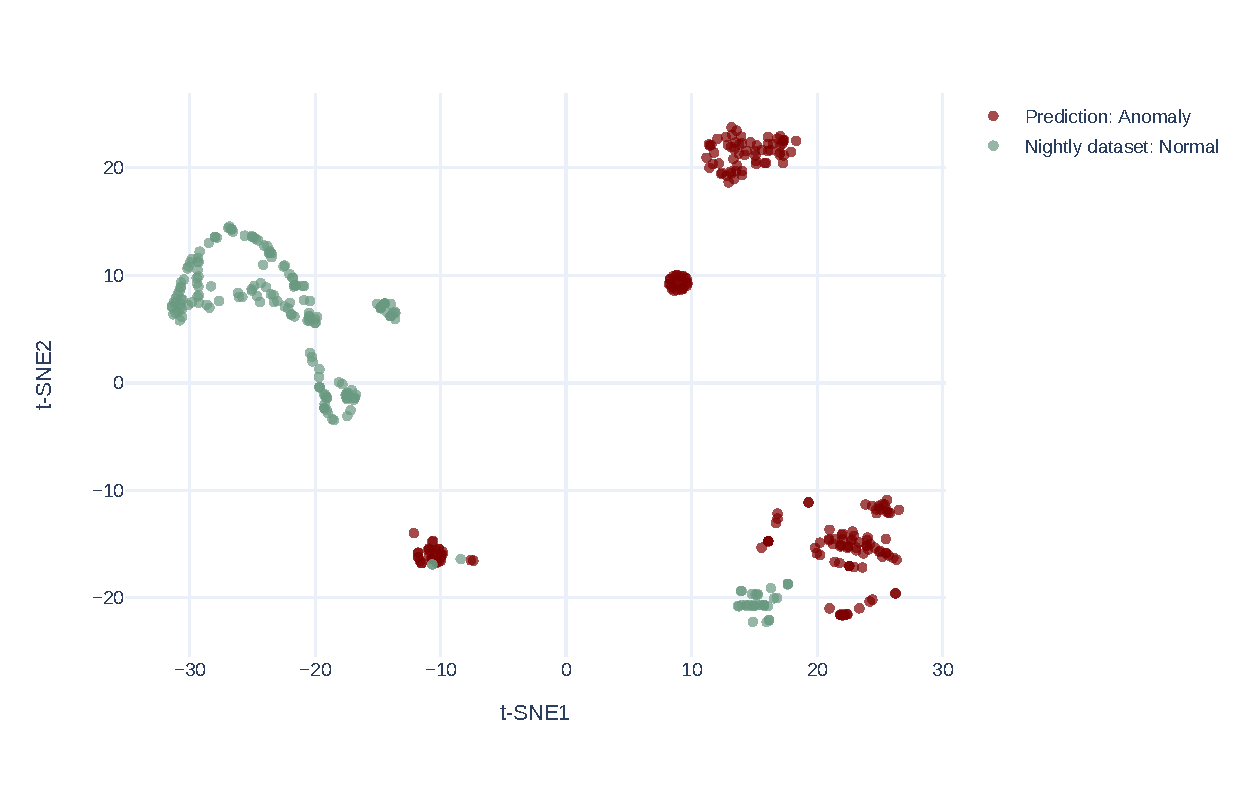
\includegraphics[width=0.9\textwidth]{img/tsne-predictions-unlabeled-invariants-mining.pdf} }}%
    \caption{Comparison of t-SNE applied on Isolation Forest (a) and Invariants Mining (b) predictions on the unlabeled Daily dataset. Green data points represent the normal datapoints as a point of reference, data points highlighted in blue and red represent predictions of normal or anomalous log sequence respectively.}%
    \label{fig:tsne-unlabeled-plots-appendix}%
\end{figure}

\begin{figure}%
    \centering
    \subfloat[\centering Isolation Forest]{{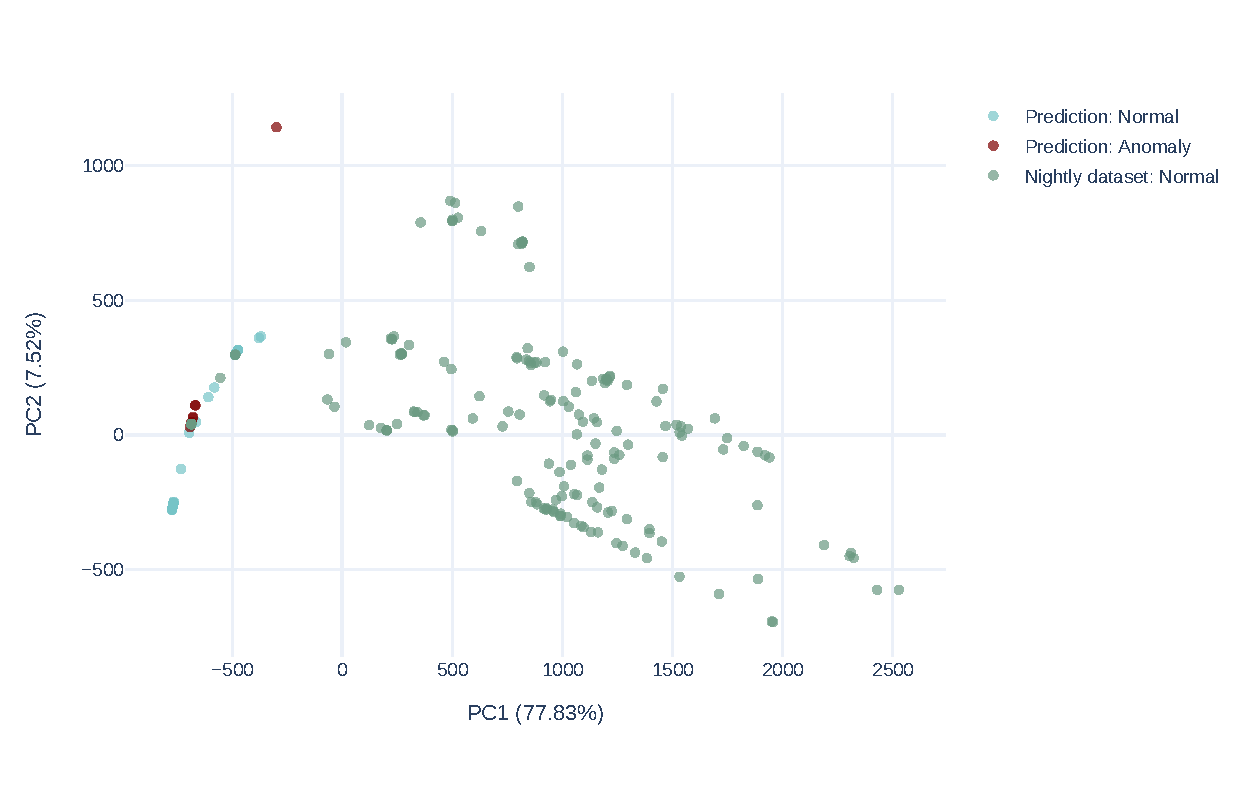
\includegraphics[width=7cm]{img/pca-predictions-unlabeled-isolation-forest.pdf} }}%
    \qquad
    \subfloat[\centering PCA]{{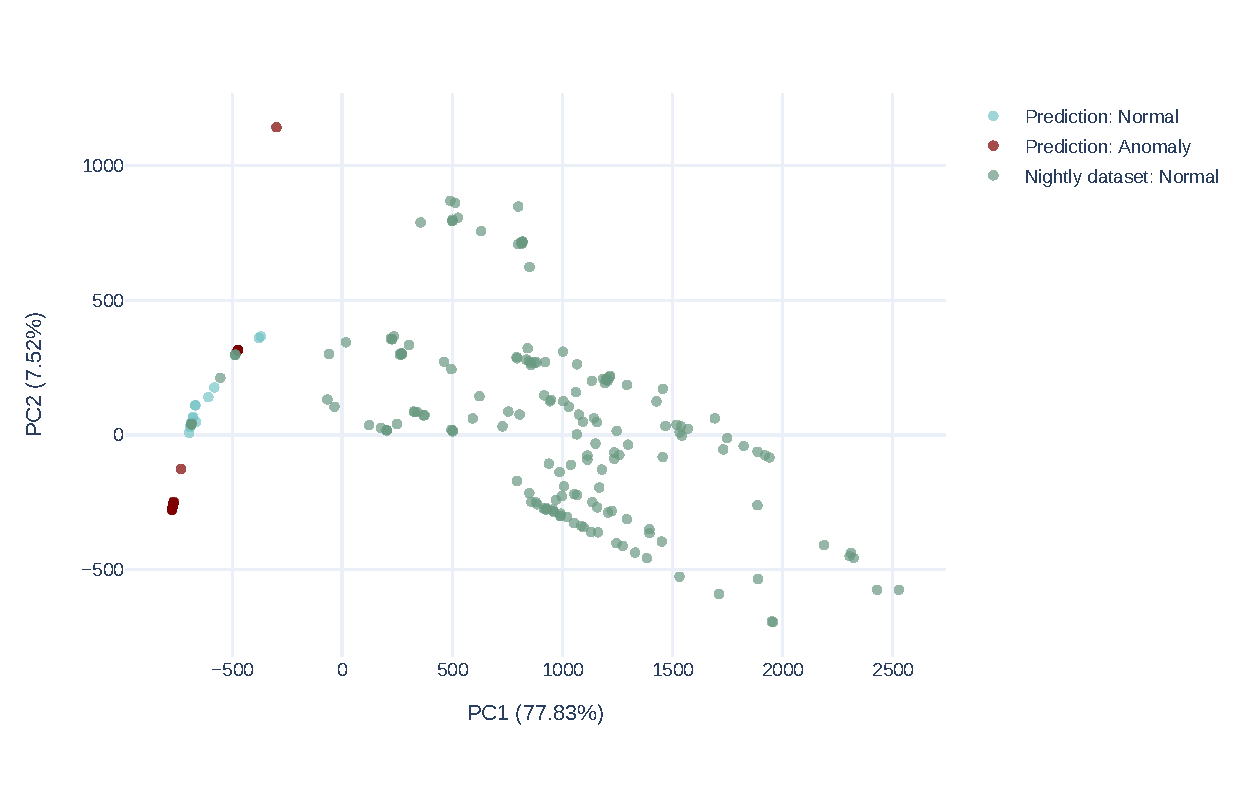
\includegraphics[width=7cm]{img/pca-predictions-unlabeled-pca.pdf} }}%
     \qquad
    \subfloat[\centering Invariants Mining]{{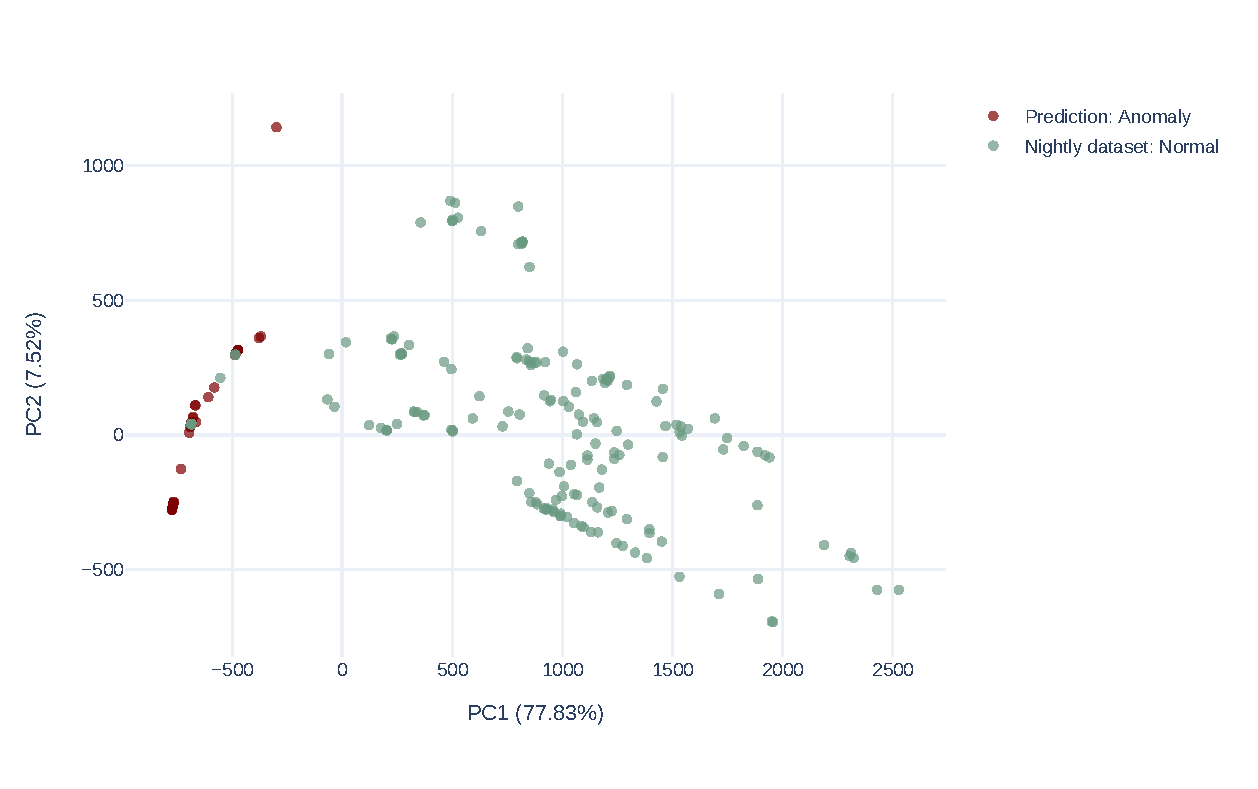
\includegraphics[width=7cm]{img/pca-predictions-unlabeled-invariants-mining.pdf} }}%
     \qquad
    \subfloat[\centering Log Clustering]{{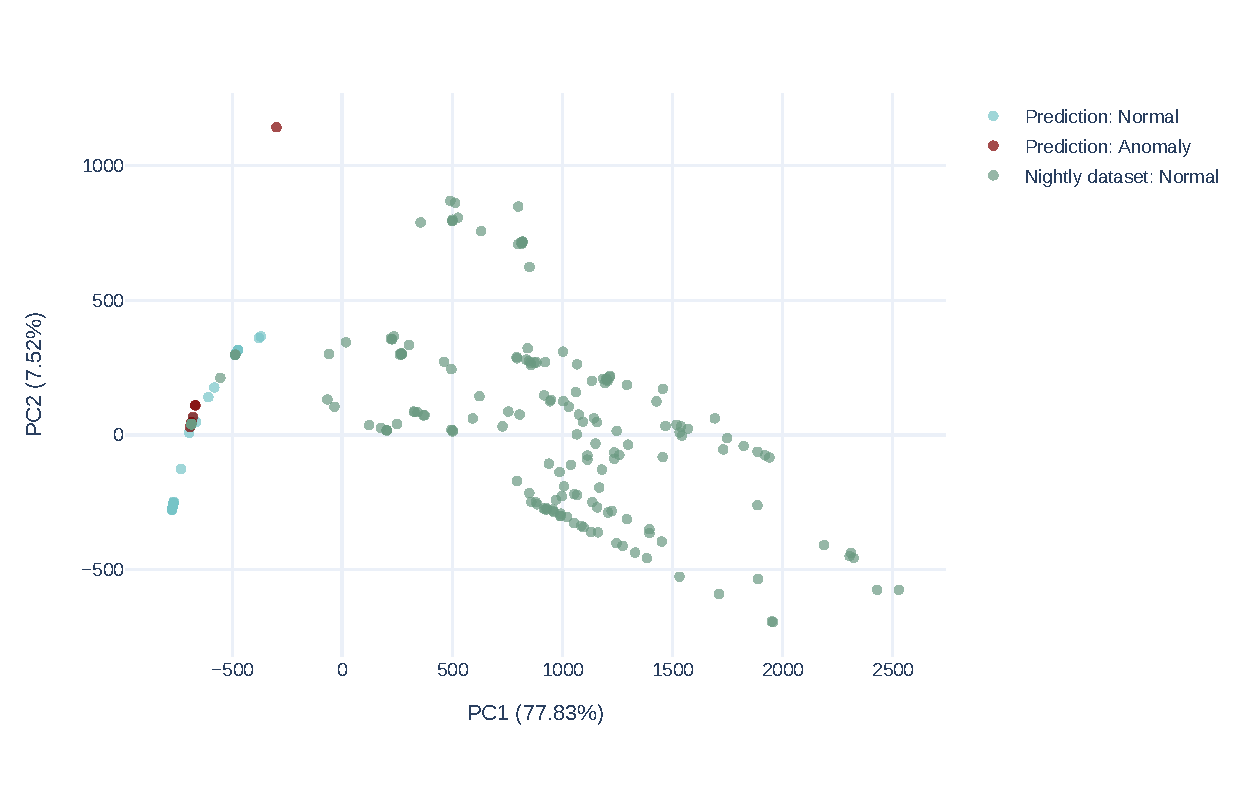
\includegraphics[width=7cm]{img/pca-predictions-unlabeled-clustering.pdf} }}%
    \caption{Comparison of PCA applied on Isolation Forest (a), PCA (b), Invariants Mining (c) and Log Clustering (d) predictions on the unlabeled Daily dataset. Green data points represent the normal datapoints as a point of reference, data points highlighted in blue and red represent predictions of normal or anomalous log sequence respectively.}%
    \label{fig:pca-unlabeled-plots-appendix}%
\end{figure}